%%%%%%%%%%%%%%%%%%%%%%%%%%%%%%%%%%%%%%%%%%%%%%%%%%%%%%%%%%%%%%%%%%%%%%%%%%%%%%%%
%2345678901234567890123456789012345678901234567890123456789012345678901234567890
%        1         2         3         4         5         6         7         8
% THESIS Chapter

\label{chap:second}
\ifpdf
    \graphicspath{{Chapter1/Figures/PNG/}{Chapter1/Figures/PDF/}{Chapter1/Figures/}}
\else
    \graphicspath{{Chapter1/Figures/EPS/}{Chapter1/Figures/}}
\fi



\section{Remote sensing and SAR imaging}
\label{sec:sar_image_formation}
Remote Sensing (RS) is the science of obtaining and interpreting information from a distance using sensors that are not in physical contact with the object being observed. Through remote sensing it is possible to study several processes that occur on Earth. For example, remote sensing has applications in geology, oceanography, meteorology, forest monitoring and even monitoring urban areas subsidence. Physically, remote sensing works by transmitting and receiving electromagnetic waves, and by studying the reflected waves, it is possible to extract parameters about the process of interest.
There are two classes of remote sensing: Passive RS and Active RS. Passive RS works by receiving natural radiation emitted or reflected by Earth, while active RS uses sensors that produces their own electromagnetic radiation (e.g.,RADAR).

The Synthetic Aperture Radar (SAR) is an active RS sensor that has several applications in the modern world and several advantages. Two major advantages is that it is possible to monitor the Earth 24 hours per day and it has little dependence of weather conditions while optical sensors can only be used at daylight and cannot be used for monitoring if there are clouds in the area at the time of the study.

A SAR is a side looking radar used in remote sensing for imaging purposes. 
It consists of an antenna mounted on a spaceborne or airborne platform, that transmits sequentially electromagnetic waves to the Earth's surface. The backscattered echoes are then collected by the same antenna a fraction of a second after the transmission. In a SAR the time of transmission of the pulse and the time of reception of the pulse are related to different antenna positions due to the platform movement. By coherent combination of the received echoes it is possible to synthesize a virtual aperture that is much greater than the antenna length. This basic principle of a SAR is what gives origin to the name ``synthetic aperture" and makes possible for the SAR to be an imaging radar. The image obtained is just a reflectivity scene of the area, that due to the coherent property of the SAR, allows to record amplitude and phase of the received signal. For a more detailed explanation regarding SAR it is recommended \cite{livro}.

Figure 1.1 demonstrates the basic geometry for image acquisition of a SAR. The flight direction is called the along-track dimension and is also called the azimuth direction. The $x$ axis is called the across-track direction or the ground range direction. The slant range (also called range) direction is the direction between the sensor and the target point on the ground.\\
The sensor is an antenna with length $L_a$ along the azimuth direction.

\begin{figure}[H]
    \centering
    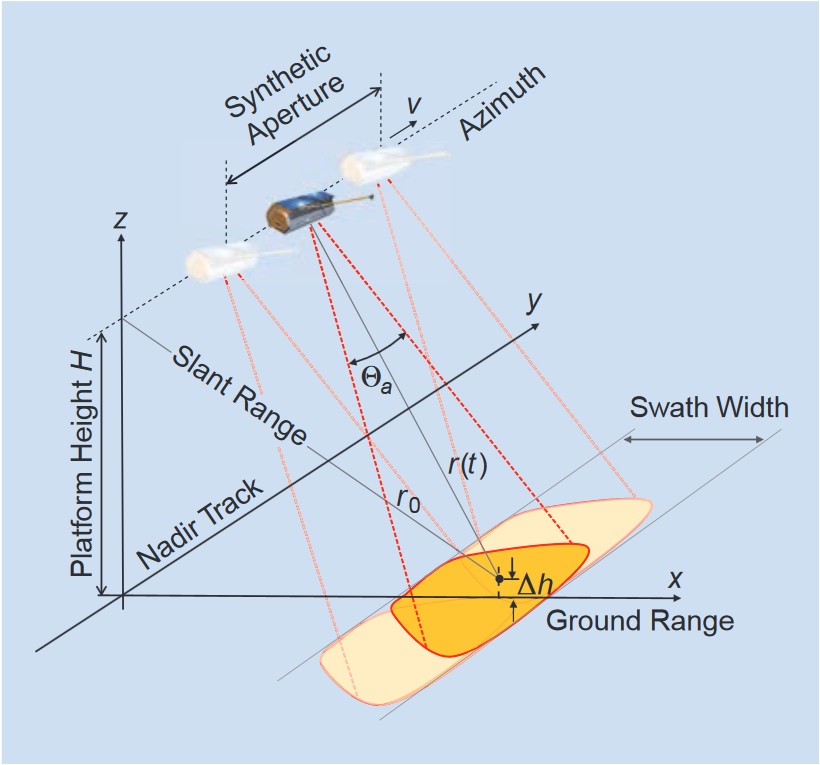
\includegraphics[width=0.8\linewidth]{Cap1/geometry.png}
    \caption{Illustration of SAR geometry. $r_0$ is the shortest distance to target, $\theta_a$ stands for the azimuth beam width and $v$ for the satellite speed. \cite{tutorial}}
    \label{fig:SAR_geometry}
\end{figure}{}

The resolution of an image in a given direction is the minimal distance between two points so it is still possible to identify the two different points on the image (also called to resolve the two different targets). In SAR there are resolution on range direction and azimuth direction, which is the minimal distance to separate two targets on range direction and azimuth direction respectively.\\
For resolving two separate targets, it is normally considered that the spatial separation of the pulses should be higher than half of the Bandwidth of the pulse (this is visually explained in \figref{fig:pulse_separation}).

\begin{figure}[H]
    \centering
    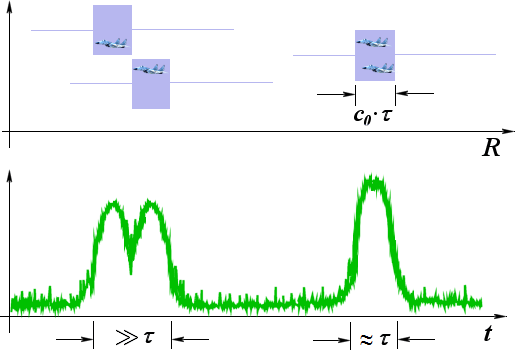
\includegraphics[width=0.8\linewidth]{Cap1/ra1_print.png}
    \caption{Temporal separation of pulses for target resolution. $\tau$ is the pulse temporal width.}
    \label{fig:pulse_separation}
\end{figure}{}

From \figref{fig:pulse_separation}, it is possible to understand why it was adopted that the temporal separation should be greater than half $\tau$. If it is greater it's reasonable to assume that it is possible to separate the targets, but if it is less than that then it's not clear the target separation.

For SAR systems, the resolution in azimuth is equal to half the antenna length. And the resolution in range direction is given by: 

\begin{equation}
    \rho_{rg} = \frac{c\tau_{rg}}{2} = \frac{c}{2B_{rg}}
\end{equation}
where $\rho_{rg}$ is the range resolution, $c$ is the speed of the light, $\tau_{rg}$ is the temporal resolution and $B_{rg}$ is the bandwidth.

After acquiring the image of the area, it is necessary to filter the image, so it is clearer for interpretation and information extraction. This is done by using two matched filters (to maximize the signal-to-noise ratio of the image), one in the azimuth direction and the other in the range direction. 
This process of applying these two filters is called range compression and azimuth compression.

\figref{fig:sar_compression} gives a summary of how the azimuth and range compression works. The focusing process is done by making convolutions (usually carried out in frequency domain) with the reference function for the received signal in the range direction and in the azimuth direction.
\begin{figure}[H]
    \centering
    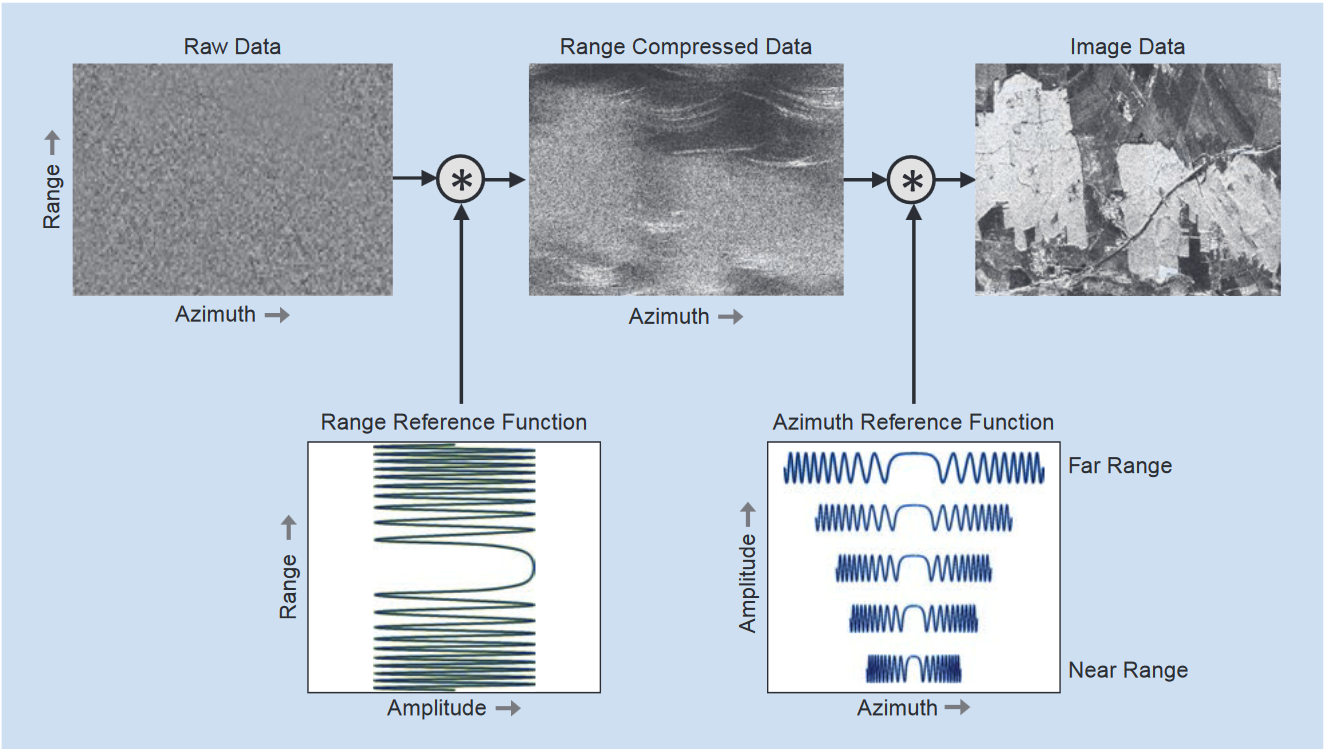
\includegraphics[width=\linewidth]{Cap1/compres.png}
    \caption{Summary of SAR compression in range and azimuth directions. \cite{tutorial}}
    \label{fig:sar_compression}
\end{figure}

After the compression process it is finally obtained a complex matrix called Single Look Complex (SLC) matrix. The amplitude of each element of this SLC matrix represents the power reflected to the antenna. After the compression, it is possible to obtain the backscatter coefficient by multiplying the absolute value of the SLC by a calibration constant obtained experimentally.
The backscatter value acquisition is important because accurate backscatter values enable more accurate results in applications like deforestation monitoring, land-cover classification and delineation of wet snow covered area \cite{Small}. It is also important to mention that the local terrain has an important role in the determination of the backscatter value, and if a Digital Elevation Model (DEM) of the area is not available then the final result might be compromised.

According to \cite{Small} the radar backscatter $\beta$ is expressed as the ratio between scattered power $P_s$ and incident power $P_i$ at ground level: $\beta = \frac{P_s}{P_i}$. When one chooses a reference area $A_\beta$ in the slant range plane, it is possible to define the radar brightness or  $\beta^0$ backscatter according to \cite{Raney} as $\beta^0 = \frac{\beta}{A_\beta}$.

If the reference area is the ground area ($A_\sigma$), then the result is the \textit{sigma naught} and it is defined as $\sigma^0 = \frac{\beta^0 \cdot A_\beta}{A_\sigma} = \beta^0 \cdot \sin(\theta)$:


Instead, if the reference area is perpendicular to the line of sight $A_\gamma$, then the \textit{gamma naught} $\gamma^0$ is the result:

\begin{equation}
    \gamma^0 = \frac{\beta^0 \cdot A_\beta}{A_\theta} = \beta^0 \cdot \tan(\theta)
\end{equation}{}

A visual description of these normalized backscatter coefficients is shown in \figref{fig:normalization_areas}

\begin{figure}[H]
    \centering
    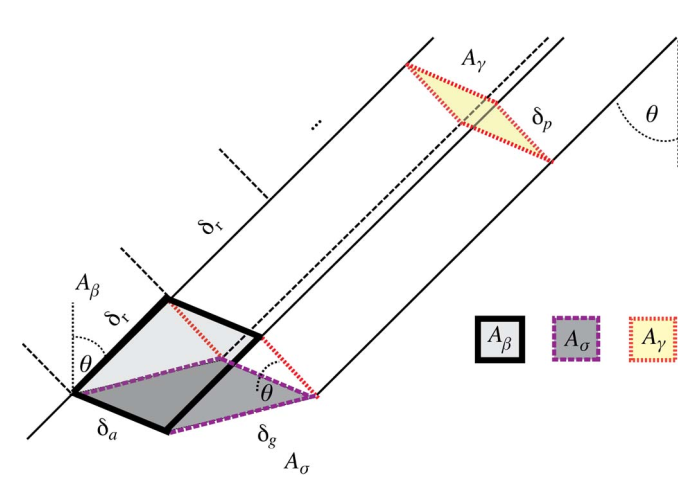
\includegraphics[width=0.8\linewidth]{Cap1/retang.png}
    \caption{Normalization areas for SAR backscatter. \cite{Small}}
    \label{fig:normalization_areas}
\end{figure}


\subsection{SAR Image Geocoding}
\label{sec:sar_geocoding}

When an image of a SAR is acquired, there is no direct correspondence on the coordinates $(x,y,z)$ on the ground reference, since the coordinates of a pixel are in coordinates of range and azimuth. The process of transforming a SAR image from range and azimuth coordinates to local cartesian coordinates on the ground is called geocoding. By using the SAR image acquired, and a reference Digital Elevation Model of the area it is possible to find the points of the SAR image that correspond to the points of the Earth model used as a reference. It is important to make clear that it is absolutely necessary a DEM of the area since a SAR image is a 2D photo of a 3D area, and therefore it is not possible to make the inversion of coordinates since information is lost when making the image acquisition.

\section{SAR Interferometry}
\label{sec:sar_interferometry}
The SAR interferometry process uses the fact that two points on the ground with different heights when looked at two distinct positions in the plane perpendicular to the azimuth direction, will give a change in the phase difference of the received signal coming from these points.\\
By comparing acquisitions obtained at different antennas positions it is possible to extract additional information of a scene. The first time this was done was in 1974 by Graham \cite{Graham}, who obtained a pattern of interference fringes by vectorially adding the signals received from two SAR antennas.
One very important remark shown by \cite{Graham} is that the type of information extracted depends on the implementation of the system. If the images are acquired at different positions but at the same time, then it is possible to extract information about the topography of the area: this is called the across-track SAR interferometry (XTI-SAR). On the other hand, if the images are taken at different times it is possible to get a map of the surface velocities: this technique is called Differential InSAR(D-InSAR).


By taking the product of the first image with the conjugate of the second image it is possible to obtain the interferogram of that area. This interferogram is still not very useful for information extraction since there are more factors that affect the interferogram that must be compensated.
The first step important is the flat earth component removal of the interferogram, which is compensate the effect of the phase added to the interferogram due to the horizontal distance of the target. After the flat earth removal what is left is called the interferometric phase. \cite{Rosen} and \cite{Bamler} give a summary of how to compensate the flat earth component of the interferogram.


There are two kind of acquisitions that can be used for extracting inteferometric information.
\begin{itemize}
    \item 
    Repeat-pass interferometry: Where the images are acquired during different passes. Normally this means that there are a temporal interference and the quality is inferior, since it is subject to changes in the scene, atmospheric changes.
    \item
    Single-pass interferometry: Where the images are acquired at the same time. This means that the quality of the interferogram is superior, since there are less factors that can affect the final product. Since the temporal decorrelation does not affect this type of interferogram, it is chosen as the product for creation of a Digital Elevation Model (DEM) due to its superior quality.
\end{itemize}

\subsection{Height acquisition and interferogram equations}
Consider two SAR images acquired over the same area using sensors S1 and S2. The distance of the sensors is called the baseline $B$. Its projections, perpendicular and parallel to the slant range dimension, are the normal baseline $B_{\perp}$ and the parallel baseline $B_{\parallel}$, respectively. They are oriented at an angle $\beta$ with respect to the local horizontal.

\begin{figure}[H]
    \centering
    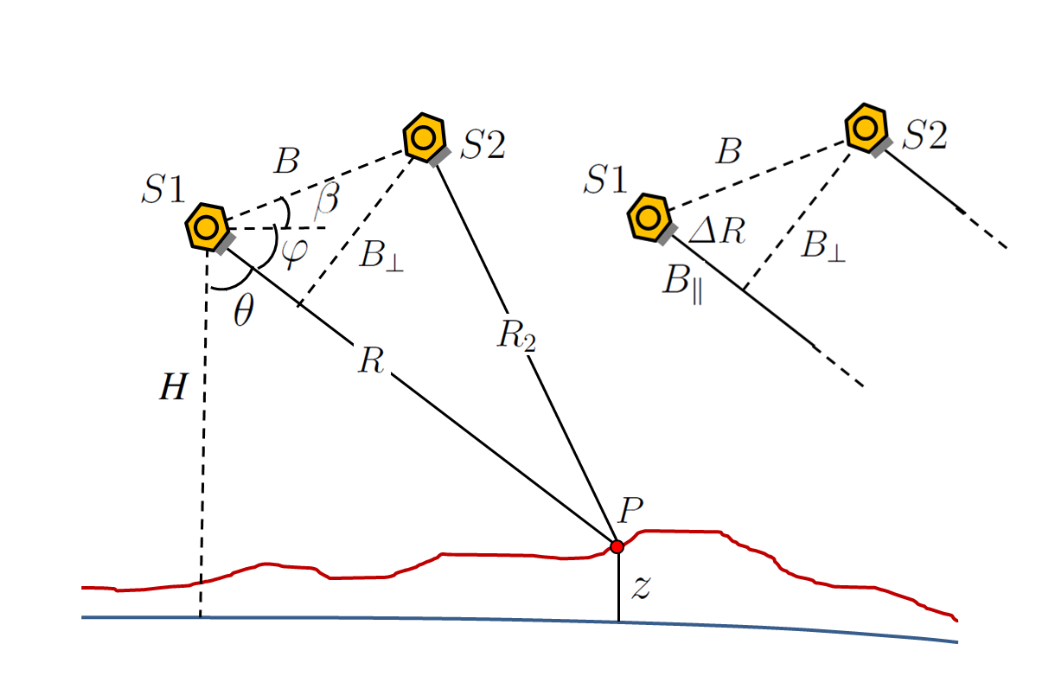
\includegraphics[width=\linewidth]{Cap1/int.png}
    \caption{Reference geometry for across-track interferometry. \cite{Paolathesis}}
    \label{fig:reference_geometry}
\end{figure}

Since the slant-range distance is normally much greater than the baseline the following approximation holds true: $|R - R_2| \ll R$, where R is the distance from the Sensor S1 to the point on ground, R2 is the distance from sensor S2 to the point on ground.

The angle $\varphi$ is given by $\varphi = \frac{\pi}{2} - \theta$, 
and by applying the cossine law on triangle S1 S2 P it yields:
\begin{equation}
    (R-\Delta R) ^2 = R^2 + B^2 - 2BR \cos(\varphi + \beta)
\end{equation}

Using the parallel-ray aprroximation we get the following result:
\begin{equation}
    \Delta R = B \sin(\theta - \beta)
\end{equation}

And the topographical height $z$ is obteined as: 
\begin{equation}
    z = H - R\sin(\varphi)
\end{equation}
where $H$ is the height of S1.

By assuming a monostatic configuration (where both sensor acquire independently an image of the same area) we get 
finally that the phase of a pixel within the SAR image on sensor S1 is:
\begin{equation}
    \Phi_1 = -\frac{4\pi}{\lambda} R + \Phi_{obj,1}
\end{equation}
and the phase of a pixel within the SAR image on sensor S2 is:
\begin{equation}
    \Phi_2 = -\frac{4\pi}{\lambda} (R - \Delta R) + \Phi_{obj,2}
\end{equation}
where $\Phi_{obj,1}$ and $\Phi_{obj,2}$ are the phases in the images of Sensor S1 and S2. These phases in the images are assumed to be the same.

Therefore, the interferometric phase is obtained as the difference between the phases, such that:
\begin{equation}
    \Phi_{int} = \Phi_{1} - \Phi_{2} = -\frac{4 \pi}{\lambda} \Delta R
\end{equation}
and for a bistatic configuration (where only one radar transmits and both receive) it equals to:
\begin{equation}
    \Phi_{int} = -\frac{2 \pi}{\lambda} \Delta R
\end{equation}


Since the phase difference is half the phase difference for a bistatic configuration since the transmit path does not affect the phase difference.

The interferogram is the two dimensional image of the $\Phi_{int}$. It is worth mentioning that before the computation of the interferogram it is needed to make the coregistration of the images, that is merely to project one image on the geometry of the other image.
Once the interferogram has been computed the interferometric phase can be decomposed into two parts: the topographical phase component and the flat earth component.

\begin{equation}
    \Phi_{int} = \Phi_{topo} + \Phi_{fe}
\end{equation}
where $\Phi_{topo}$ is the topographic component and $\Phi_{fe}$ is the flat earth component.
The flat earth component accounts for the interferometric phase difference ocurring between two scatterers at the same topographical height but at different horizontal positions. The flat earth component is visually explained in \figref{fig:reference_geometry}.

\begin{figure}[H]
    \centering
    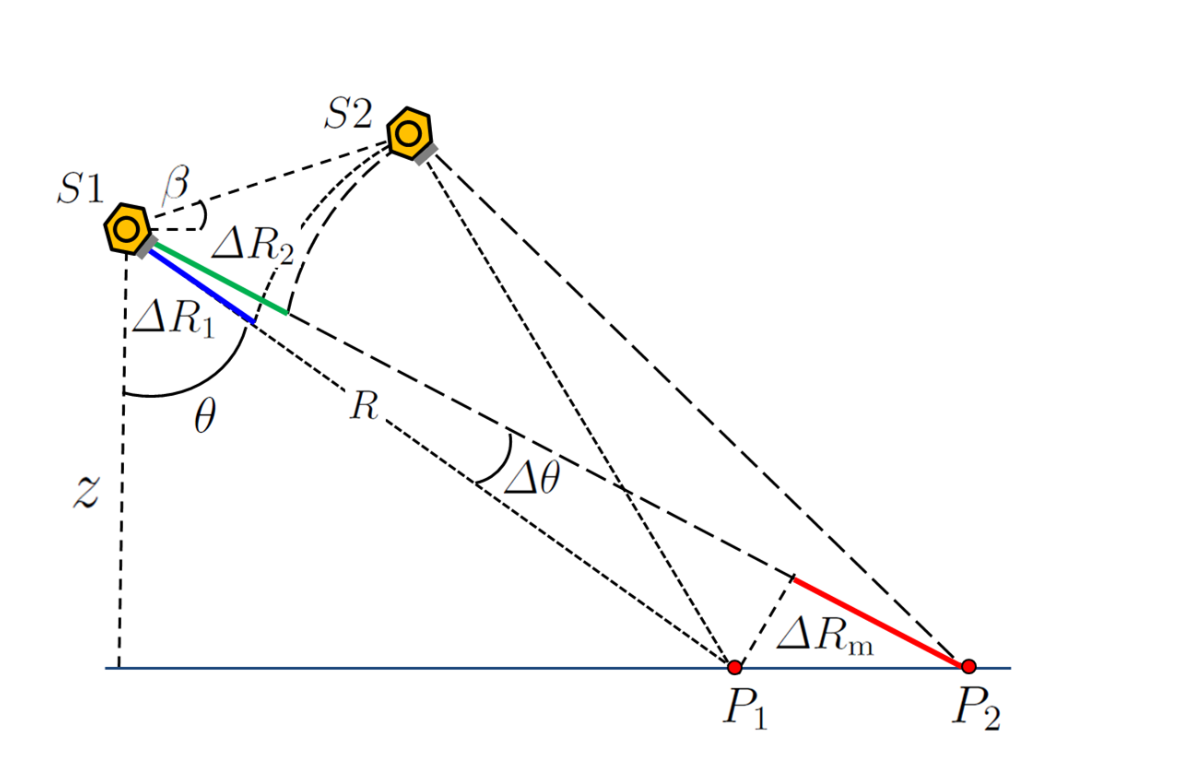
\includegraphics[width=\linewidth]{Cap1/flat.png}
    \caption{Reference geometry for flat earth component. \cite{Paolathesis}}
    \label{fig:flat_earth_component}
\end{figure}

Consider now two points $P_1$ and $P_2$ on the same topographical height. The inteferometric phase for each one is given by:
\begin{equation}
    \Phi_1 = -\frac{4\pi}{\lambda}\Delta R_1 = -\frac{4\pi}{\lambda}B_{\perp}\sin(\theta - \beta)
\end{equation}
and for P2
\begin{equation}
    \Phi_2 = -\frac{4\pi}{\lambda}\Delta R_2 = -\frac{4\pi}{\lambda}B_{\perp}\sin(\theta + \Delta \theta - \beta)
\end{equation}

The difference between the two fases is the flat earth component that should be removed. Therefore the flat earth component equals to:
\begin{equation}
    \begin{aligned}
        \Phi_{fe} = & \Phi_1 - \Phi_2 = -\frac{4\pi}{\lambda}[B\sin(\theta + \Delta \theta - \beta) - B\sin(\theta - \beta)] = \\ 
        & \frac{4\pi}{\lambda}B\cos(\theta - \alpha)\Delta \theta
        \approx \frac{4\pi B\cos(\theta - \alpha)\Delta R_m}{\lambda R \tan(\theta)}
    \end{aligned}
\end{equation}
where $R_m$ is the slant range difference between $P1$ and $P2$.

The results of the extraction of the flat earth component can be visualized in the figure below.
\begin{figure}[H]
    \centering
    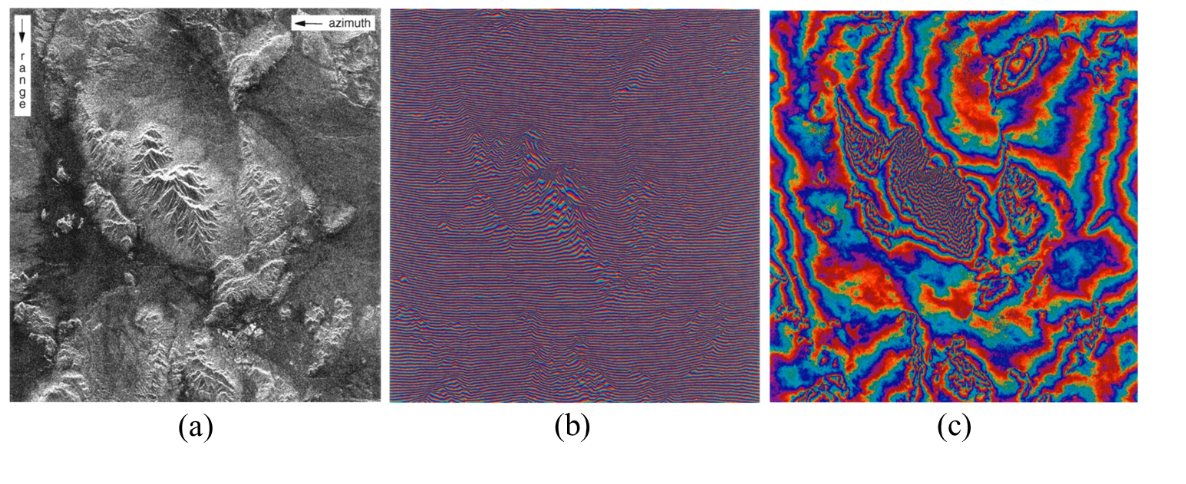
\includegraphics[width=\linewidth]{Cap1/flat_interf.png}
    \caption{(a) Amplitude of image of SAR image acquired by ERS-1/2 at C-Band with a baseline of $133$m.
    (b) Interferogram before the flat earth component removal. (c) Interferogram after the flat earth component removal. The color on the images represent the value of the interferometric phase of the pixel, such that pixels connected with the same color should have the same topographical height. \cite{Paolathesis}}
    \label{fig:flat_earth_removal}
\end{figure}


The altitude difference $h_{amb}$ corresponding to a phase variation of $2\pi$ is called height of ambiguity. It is inversely proportional to the perpendicular baseline $B_{\perp}$ and is defined as:
\begin{equation}
    h_{amb} = \frac{\lambda R \sin(\theta)}{nB_{\perp}}
\end{equation}
where $n=2$ for monostatic configuration and $n=1$ for a bistatic configuration.
The idea is that the higher the perpendicular baseline the lower the height of ambiguity and therefore the more accurate the height estimation is.

It is also important to mention the process of phase unwrapping for the processing of the topographical phase component.\\
Since the topographical phase obtained is modulo $2\pi$ it is important to reconstruct the correct phase by adding multiples of $2\pi$ to the phase obtained. 
This process is called phase unwrapping and it is show in Figure 1.8.

\begin{figure}[H]
    \centering
    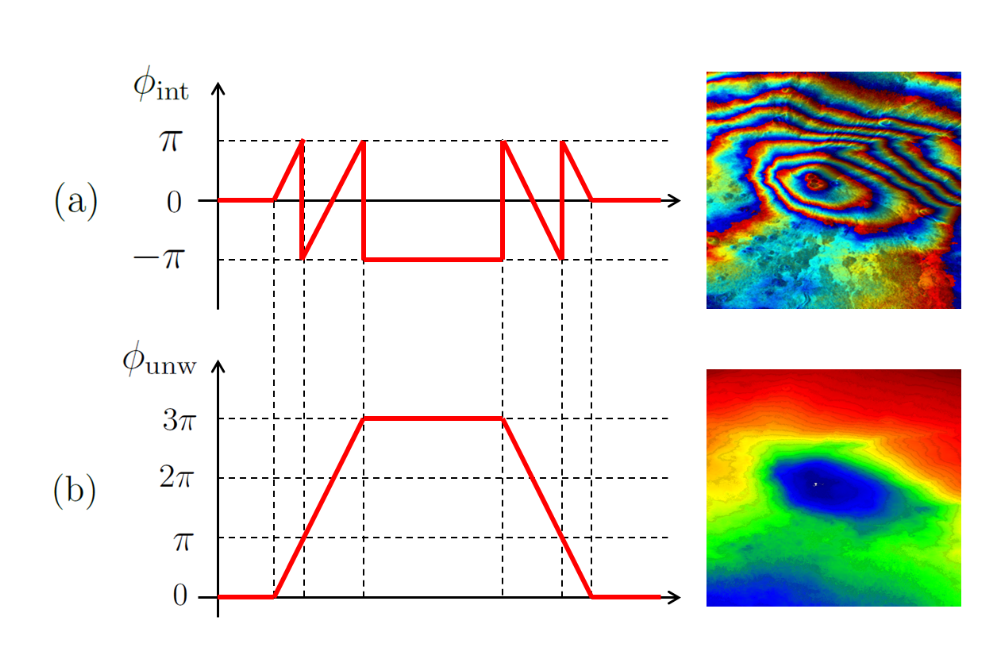
\includegraphics[width=\linewidth]{Cap1/unwr.png}
    \caption{Explanation about phase unwrapping. 
    (a) Topographical phase before the phase unwrapping.
    (b) Topographical phase after the unwrapping of the phase.
    The images are obtained from a repeat pass acquisition SIR-C-X SAR over Mount Etna, Italy. \cite{Paolathesis}}
    \label{fig:phase_unwrapping_process}
\end{figure}

After the flat earth removal and phase unwrapping the interferogram is finally ready for analysis and information extraction.

\subsection{The Complex Interferometric Coherence}
The interferometric coherence($\gamma_t)$ is a measure of the quality of the interferogram. It is, for each pair of corresponding pixels, the correlation between these two pixels: $u_1$ and $u_2$. It is given by:
\begin{equation}
    \rho = \frac{E[u_1u_2^*]}{\sqrt{E[|u_1|^2]E[|u_2|^2]}}
\end{equation}{}
where $E[\cdot]$ is the expectation operator. In practice it is not possible to obtain the correlation between the random variables that model the complex value of the pixels, so in practice this correlation is obtained by a moving average filter along the image.
What is obtained is then a estimation of the real value of the coherence, by using this moving average filter what is obtained is the Maximum Likelihood Estimation of the coherence. This is obtained as:
\begin{equation}
    \rho_{MLE}[i,j] = \frac{\sum_{i=1}^N[u_1[i]u_2^*[i]]}
    {\sqrt{\sum_{i=1}^N|u_1[i]|^2\sum_{i=1}^N|u_2[i]|^2}}
\end{equation}{}
Where $N$ is the number of independent samples used to compute the coherence estimation. 
The absolute value of the coherence, gives information about the decorrelation level and it is also a measure of the quality of the interferogram. The phase of the coherence, also called interpherometric phase, gives information about the path difference between the two antennas used for the acquisition. 

It is important to say that this estimation of the coherence is not unbiased, even though it is asymptotically unbiased \cite{Bamler}. In fact, if the values of the pixels are assumed to follow a gaussian distribution, then it is possible to find the relationship between the estimated coherence, the real value of the coherence and the number of samples used to make the estimation. This function is show in \figref{fig:bias}.

\begin{figure}[H]
    \centering
    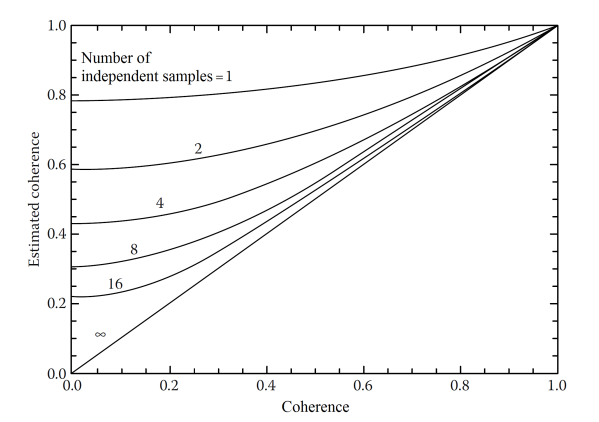
\includegraphics[width=\linewidth]{Cap1/bias.png}
    \caption{Bias of the MLE coherence estimator. \cite{Bamler}}
    \label{fig:bias}
\end{figure}

It is important to notice that the estimator is always biased towards higher values than it actually is, and by increasing the number of samples the estimation gets every time closer to the real value. It is also important to notice that for high values of the coherence the estimator provides a better estimation than it would if the coherence were of low value. 

This coherence number is crucial to the textures work that will be developed on the rest of the work, since there is much useful information for classification that can be extracted by looking at this number and by making the textures of the coherence image.

\subsection{Co-registration}
Before taking the complex interferometric coherence between the images, a step called co-registration is necessary. After making the focusing step of the two images, it is necessary to transform the slave image to what it would look like if it was taken with the acquisition geometry of the master image. Since the images are taken with different geometries, it produces effects of rototranslations that can scale differences between the images and induce errors in the coherence process. Therefore, this co-registration is a process that correctly alligns the two images to the same geometry and reduces the effects of errors in the calculation of the interferometric coherence\cite{andreathesis}.

\subsection{Decorrelation in Vegetated Areas}
According to \cite{Martone} different factors contribute to the total coherence and the coherence can be written as a product of the different contributions to the coherence as follows:

\begin{equation}
    \rho =\rho_{SNR}\cdot\rho_{Quant}\cdot\rho_{Amb}\cdot\rho_{Range}\cdot\rho_{Azimuth}\cdot\rho_{Vol}\cdot\rho{Temp}
\end{equation}

The terms on the right hand side describe the errors contribution due to: limited Signal to noise ratio ($\rho_{SNR}$), quantization errors($\rho_{Quant}$), ambiguities($\rho_{Amb}$),
baseline decorrelation 
($\rho_{Range}$), errors due to relative shift of the doppler spectra 
($\rho_{Azimuth}$), and temporal decorrelation($\rho_{Temp}$). 

The term ($\rho_{Vol}$) is the volume correlation factor and it is due to volume scattering. On forests this is mainly due to vegetation and therefore is crucial for forest land-cover classification.\\

A more detailed explanation about each contribution to the coherence is given by \cite{Martone2} and \cite{Rizzoli}, but a summary of each contribution is given following:

\begin{itemize}
    \item
    $\rho_{SNR}$: Is the coherence loss due to finite sensitivity of the radar system. It can be calculated from the Signal to Noise Ratio of the SAR System as follows:
    \begin{equation}
        \rho_{SNR}=\frac{SNR}{1+SNR}
    \end{equation}{}
    According to \cite{Martone3} for the TANDEM-X satellite system is holds that: \newline
    $\rho_{SNR}>0.8$
    \item
    $\rho_{Quant}$: It represents the error due to quantization of the recorded received signal. From \cite{Martone2} it is expected that this value is lower than 10\%.
    \item
    $\rho_{Range}$: Possible baseline decorrelation effects are estimated by deriving a local slope map from orbit and elevation information.
    \item
    $\rho_{Temp}$: Is the decorrelation due to the temporal baseline between both acquisitions. On TANDEM-X, since both acquisitions are taken almost at the same time it holds that $\rho_{Temp}\approx 1$.
    \item
    Also according to \cite{Martone3} and \cite{Krieger} the contributions of $\rho_{Amb}$ and $\rho_{Azimuth}$ are very small (less than 2\%) and are solved in the TANDEM-X by adaptative selection of the azimuth processing bandwidth and total independent zero Doppler steering.
\end{itemize}

In \cite{Krieger} there is a more detailed explanation about the different correlation factors.


In \cite{Paolo} it was also shown that a study about the evolution of the temporal correlation of an area can also provide useful information for land-cover classification. The temporal decorrelation is modelled in \cite{Paolo} as:
\begin{equation}
    \rho_{Temp} = (1-\rho_{LT})e^{-(\frac{t}{\tau})^2} + \rho_{LT}
\end{equation}{}
where $\gamma_{LT}$ is the long term coherence, $t$ is the time and $\tau$ is the target decorrelation factor. The determination of these parameters also provide  important information that might help improve the land cover classification algorithms. The work developed in \cite{Paolo} is crucial for this thesis, since this thesis is strongly based on this work and it lays the foundation for an improvement of land cover classification that is proposed on the end of this work.


